\documentclass[12pt]{article}

\newcommand{\documento}{Piano Di Qualifica}
\usepackage{titling}
\usepackage{caption}
\usepackage{multirow}
\usepackage[T1]{fontenc}
\usepackage[utf8]{inputenc}
\usepackage[italian]{babel}
\usepackage{tabularx}
\usepackage [colorlinks=true,urlcolor=blue, linkcolor=black]{hyperref}
\newcommand{\subtitle}[1]{%
  \posttitle{%
    \par\end{center}
    \begin{center}\LARGE#1\end{center}
    \vskip0.5em}%
}

\setlength{\oddsidemargin}{0in}
\setlength{\evensidemargin}{0in}
\setlength{\topmargin}{0in}
\setlength{\headsep}{-.25in}
\setlength{\textwidth}{6.5in}
\setlength{\textheight}{8.5in}

\font\myfont=cmr12 at 40pt

\newcommand{\red}{\mic}
\newcommand{\verp}{TBD}
\newcommand{\vers}{TBD}
\newcommand{\res}{TBD}
\newcommand{\version}{Versione 0.0.0}
\newcommand{\use}{Esterno}
\usepackage{eurosym}
\title{\myfont{Piano di Qualifica}}
\author{Dream Corp.}


\setcounter{tocdepth}{4}
\setcounter{secnumdepth}{4}
\usepackage[table,xcdraw]{xcolor}
\usepackage{float}
\usepackage{wrapfig}
\usepackage{appendix}
\usepackage{amsmath, tabu}
\graphicspath{{immagini/}}
\date{\myfont 04-12-2018}

\begin{document}

	\maketitle
	\begin{center}
	
\includegraphics[width = 80mm]{../../logo.png}\newline
	\huge \version 
	\\G\&B
	
	\begin{table}[h!]
		\centering
		\begin{tabular}{r|l}
			\multicolumn{2}{c}{Informazioni sul documento}\\
			\hline
			Versione & \version \\
			Redazione & \red \\
			Verifica & \verp\\
			& \vers\\
			Responsabile & \res\\
			Uso & \use\\
			Destinatari & Dream Corp. \\
			& Zucchetti SpA\\
			& Prof. Tullio Vardanega\\
			& Prof. Riccardo Cardin\\
		\end{tabular}
	\end{table}
	
	\end{center}
	\newpage
	\medskip
\begin{table}[h!]
	\centering
	\renewcommand{\arraystretch}{2} 
	\rowcolors{2}{gray!25}{white}
	\begin{tabular}{|r|r|p{6cm}|l|l|}
		\rowcolor{orange!50}		
		\hline
		\textbf{Versione} & \textbf{Data} & \textbf{Descrizione} & \textbf{Autore} & \textbf{Ruolo}\\
		\hline
		0.6.0 & 9/01/2019 & Consuntivo di periodo e preventivo a finire & \pie & Responsabile \\
		\hline
		0.5.3 & 17/12/2018 & Preventivo validazione e totali & \pie & Responsabile \\
		\hline
		0.5.2 & 15/12/2018 & Preventivo progettazione di dettaglio & \pie & Responsabile \\
		\hline
		0.5.1 & 14/12/2018 & Preventivo progettazione architetturale & \pie & Responsabile \\
		\hline
		0.5.0 & 13/12/2018 & Preventivo avvio e analisi & \pie & Responsabile \\
		\hline
		0.4.0 & 13/12/2018 & Analisi dei Rischi & \daG & Analista \\
		\hline
		0.3.1 & 12/12/2018 & Inserimento diagrammi di Gantt & \pie & Responsabile \\
		\hline
		0.3.0 & 11/12/2018 & Scrittura pianificazione & \pie & Responsabile \\
		\hline
		0.2.0 & 05/12/2018 & Scrittura modello di sviluppo  & \daG & Responsabile \\
		\hline
		0.1.0 & 30/11/2018 & Scrittura introduzione & \daG & Responsabile \\
		\hline
		0.0.1 & 26/11/2018 & Creazione struttura del documento & \daG & Responsabile  \\
		\hline
	\end{tabular}
\end{table}
	~\newpage
	\newpage
	\tableofcontents
	\newpage

\section{Informazioni sul documento}
\subsection{Scopo del documento}
 Col fine di mantenere alta la qualità del prodotto finale il gruppo Dream Corp. ha stilato questo documento che descrive i metodi con cui analizzerà e verifichierà i processi attuati.
 \subsection{Scopo del progetto}
 Lo scopo è quello di creare un Plugin\pedice per Grafana\pedice per integrare metodi di intelligenza artificale al flusso dei dati raccolti con lo scopo di monitorare lo stato del sistema e migliorare il sfotware utilizzato
 \subsection{Glossario}
 In questo documento sono presenti termini di non immediata comprensione. Con lo scopo di disambiguare quest'ultimi è stato redatto un glossario, segnalati con una G a pedice.

 \newpage
 \subsection{Riferimenti}
 \subsubsection{Riferimenti normativi}
 \begin{itemize}
 	\item \textit{Norme di progetto};
 	\item Standard ISO/IEC 9126:
 		\begin{itemize}
 			\item[-] Modello di qualità;
 		\end{itemize}
	\item Slide del corso di "Ingegneria del Software" - Qualità del Software: \\
		\url{https://www.math.unipd.it/~tullio/IS-1/2018/Dispense/L13.pdf}
	\item  Slide del corso di "Ingegneria del Software" - Qualità di Processo: \\
		\url{https://www.math.unipd.it/~tullio/IS-1/2018/Dispense/L14.pdf}
 \end{itemize}
\subsubsection{Riferimenti informativi}
 \begin{itemize}
 	\item Slide del corso di "Ingegneria del Software" - Qualità del Software: \\
		\url{https://www.math.unipd.it/~tullio/IS-1/2018/Dispense/L13.pdf} 
	\item Qualità del software: \\
		\url{https://it.wikipedia.org/wiki/Qualità_del_software}
		\begin{itemize}
			\item[-] Elenco di metriche utili.
		\end{itemize} 
	\item  Slide del corso di "Ingegneria del Software" - Qualità di Processo: \\
		\url{https://www.math.unipd.it/~tullio/IS-1/2018/Dispense/L14.pdf}
	\item Metriche di progetto \\
 		\url{https://it.wikipedia.org/wiki/Metriche_di_progetto}
 	\item Gulpease index: \\
 		\url{https://it.wikipedia.org/wiki/Indice_Gulpease}
 	\begin{itemize}
 		\item[-] Formula di calcolo.
	\end{itemize}
	\item Gunning Fog Index: \\
		\url{https://en.wikipedia.org/wiki/Gunning_fog_index}
		\begin{itemize}
		\item[-] Formula di calcolo.
		\end{itemize}
	\item Simple Measure of Gobbledygook: \\ 
		 \url{https://en.wikipedia.org/wiki/SMOG}
		 \begin{itemize}
		 	\item[-] Formula di calcolo.
		 \end{itemize} \clearpage
	\item Code coverage: \\ 
		\url{https://en.wikipedia.org/wiki/Code_coverage}
		\begin{itemize}
		\item[-] struttura e definizione metriche.
		\end{itemize}
\end{itemize}
\newpage
\section{Qualità di processo}
\subsection{Scopo}
\textit{"Da tubi sporchi non esce acqua pulita"}.
\newline
Con questa frase questo documento si prefigge  lo scopo di adottare la qualità di processo come esigenza fondamentale per perseguire la qualità di prodotto. Proprio per questo si è deciso di adottare il PDCA e lo standard ISO/IEC 15504 denominato SPICE. Inoltre si vuole far presente come l'insieme di questi contenuti non sia definitivo ma anzi viene incrementato durante il percorso. \textbf{Questo documento deve rispondere al cosa e non al come.}
%\subsection{Procedure di controllo}
%La qualità di processo viene suddivisa in:
%\begin{itemize}
%	\item{\textbf{Definizione:} per controllarlo e raccontarlo meglio};
%	\item{\textbf{Controllo:} perchè sia conforme alle attese e costi meno};
%	\item{\textbf{Validazione:}  per validare tramite PDCA.}
%\end{itemize}
\subsection{Processi}
Con l'obiettivo di ottenere un miglioramento continuo della qualità in un'ottica a lungo raggio e all'utilizzo ottimale delle risorse è stato adottato il ciclo di Deming o ciclo PDCA. (\textbf{LA SPIEGAZIONE DEL PDCA DOVREBBE ANDARE SULLE NORME IN UN CAPITOLO A PARTE})\newline I processi qui descritti misurano la qualità del lavoro interno, ad esempio se stiamo lavorando secondo i tempi stabiliti

\subsubsection{Definizione e Pianificazione (prc1)}
Poter controllare al meglio un processo si è scelto il modello incrementale, inoltre vengono descritte le attività e i compiti da svolgere, la pianificazione del lavoro e dei costi da sostenere . (\textbf{NON DESCRIVO I MODELLI /NON USO LE APPENDICI / IN QUESTO DOCUMENTO SI DEVE PARLARE DI QUANTITA' MISURABILI e NON DI COME CI SI ARRIVA}) Il gruppo inoltre si prefigge di rispettare i seguenti obiettivi:
\begin{itemize}
		\item{\textbf{Calendario:} assicurarsi di organizzare gli obiettivi assicurandosi del loro peso per poter rispettare le scadenze}
		\item{\textbf{Budget:} tramite le metriche descritte si cerca di allineare il budget il più possibile con gli obiettivi prefissati;}
		\item{\textbf{Standard:} definire uno standard per ogni processo al fine di facilitare il lavoro di gruppo e l'incremento continuo di ogni parte.}
\end{itemize} 
\subparagraph{Metriche utlizzate}
\href{https://it.wikipedia.org/wiki/Metriche_di_progetto}{\textbf{PRESE DA QUI}}
\begin{itemize}
	\item{\textbf{SV(Schedule Variance);}}
	\item{\textbf{BV(Budget Variance);}}
	%\item{\textbf{AC(Actual Cost)}.} serve già a calcolare budget variance
	\item{\textbf{Function Points.} }
\end{itemize}
\begin{table}[!htpb]
	\centering
	\renewcommand{\arraystretch}{2} 
	\rowcolors{2}{gray!25}{white}
	\resizebox{\textwidth}{!}{%
	\begin{tabular}{|l|l|l|}
		\hline
		\rowcolor{orange!50} 
		\textbf{Nome} & \textbf{Accettazione} & \textbf{Ottimalità} \\
		\hline
		Schedule Variance & \textgreater = -3 giorni &0 giorni \\
		\hline
		Budget Variance & \textgreater = +-15\% & \textgreater = 0 \\ 
		\hline
		Function Points & - & - \\
		\hline
	\end{tabular}
	}
	\caption{Metriche utilizzate per la Definizione e Pianificazione}
\end{table}

\subsubsection{Verifica (prc2)}
Questo processo ha lo scopo di verificare che tutti gli elementi soddisfino i requisiti necessari. In questa parte ci si prefigge di rispettare i seguenti obiettivi:
\begin{itemize}
	\item{\textbf{Commit brevi ed incisivi:} per facilitare così un'analisi ed un miglior intervento di verifica alla comparsa di un nuovo bug;}
	\item{\textbf{Commenti al codice:} ogni porzione di codice deve essere commentata così da poter essere compresa e condivisa da collaboratori diversi dall'autore.}
	\item{\textbf{Parlare di integrazione continua...forse}}
\end{itemize}
Viene così utilizzata parte dei criteri fondamentali del \textit{code coverage}
\subparagraph{Metriche utilizzate}.
\begin{itemize}
	\item{\textbf{Line coverage}(primitiva rispetto alle successive, fornisce un'idea generale)}
	\item{\textbf{Functional coverage}}
	\item{\textbf{Path coverage}}
	\item{\textbf{Condition coverage}}
	\item{\textbf{Branch coverage}}
\end{itemize}
\begin{table}[!htpb]
	%\resizebox{\textwidth}{!}{%
	\centering
	\renewcommand{\arraystretch}{2} 
	\rowcolors{2}{gray!25}{white}
	\resizebox{\textwidth}{!}{%
	\begin{tabular}{|l|l|l|}
		\rowcolor{orange!50}
		\hline
		\textbf{Nome} & \textbf{Accettazione} & \textbf{Ottimalità} \\
		\hline
		Line coverage & 90\% & 100\% \\
		\hline
		Functional coverage & 93\%(non più alto per evitare ridondanza) & 100\% \\
		\hline
		Path coverage & 96\% & 100\% \\
		\hline
		Condition coverage & 98\% & 100\% \\
		\hline
		Branch coverage & 95\% & 100\% \\
		\hline
	\end{tabular}
	}
	\caption{Metriche utilizzate per la Verifica}
%}
\end{table}
\subsubsection{Analisi e gestione dei rischi (prc3)}
Questo processo ha lo scopo di monitorare ed evitare l'insorgere di nuovi rischi durante tutto il processo di realizzazione. Ci prefiggiamo quindi i seguenti obiettivi:
\begin{itemize}
	\item{\textbf{Analisi:} ad ogni fase è necessario analizzare i possibili rischi;}
	\item{\textbf{Categorizzazione:}  definire il tipo di rischio ad esempio se è di tipo noto, prevedibile o imprevedibile per raffinare gli strumenti con cui agire;}
	\item{\textbf{Catalogo dei rischi:} al fine di individuare i rischi è utile stilare un catalogo dei rischi utilizzando la suddivisione del punto precedente.}
\end{itemize}
Vengono così utilizzate le seguenti metriche: 
\begin{itemize}
	\item{\textbf{Servizi esterni non raggiungibili}}
	\item{\textbf{Rischi non calcolati}}
	\subparagraph{nota:} per le metriche descritte in questa tabella viene utilizzato un indice numerico positivo che indica il numero di servizi esterni non raggiungibili o rischi non previsti che hanno minato temporaneamente il processo. (\textbf{non so se le note vadano qui o vadano spiegate in qualche altro documento})
\end{itemize}
\begin{table}[!htbp]
	\centering
	\renewcommand{\arraystretch}{2} 
	\rowcolors{2}{gray!25}{white}
	\resizebox{\textwidth}{!}{%
		\begin{tabular}{|l|l|l|}
			\rowcolor{orange!50}
			\hline
			Nome & Accettazione & Ottimalità \\
			\hline
			Servizi esterni non raggiungibili & 0 & 0 \\
			\hline
			Rischi non previsti & 0 & 0 \\
			\hline
		\end{tabular}
	}
	\caption{TBD}
\end{table}
\newpage
\subsubsection{Gestione Test (prc4)}
Prendendo nota che il processo di sviluppo è ancora in fase embrionale il gruppo non è ancora in grado di fornire delle metriche per la gestione dei test.
\subsubsection{Versionamento (prc5)}
Come per la gestione dei test vale anche per il processo di versionamento

\newpage
\section{Qualità del Prodotto}
\subsection{Scopo}
Qualità del software effettivo, leggibilità dei documenti (sono un prodotto anche quelli), misura dei test.
Le norme UNI definiscono la qualità come \textit{"l'insieme delle carrateristiche che gli conferiscono la capacità di soddisfare esigenze espresse o implicite"}
\subsection{Prodotti}
\subsubsection{Qualità dei documenti}
Ci si prefigge lo scopo di creare dei documenti standardizzati, per questo i nostri obiettivi sono:
\begin{itemize}
	\item{\textbf{Comprensibilià:} devono venire creati dei coumenti di immediata comprensione, per questo si prediligono frasi incisive e si pone l'accento su elementi tecnici presentati da tabelle;}
	\item{\textbf{Correttezza:} non devono contenere errori ortografici;}
	\item{\textbf{Leggibilità:} nonostante lo scopo tecnico i documenti devono essere fruibili alla maggior parte delle persone.}
\end{itemize}
\vspace{0.8cm}
%Vengono così utilizzate le seguenti metriche per poter dare un ranking ai documenti:
\subparagraph{Metriche utilizzate}
\begin{itemize}
	\item{\textbf{Gulpease Index}}
	\item{\textbf{Errori sintattici}}
	\item{\textbf{Gunning Fog index}}
	\item{\textbf{Coleman Liau index/SMOG}}
\end{itemize}
\begin{table}[!htpb]
	\resizebox{\textwidth}{!}{%
		\begin{tabular}{|l|l|l|}
			\hline
			\rowcolor[HTML]{34CDF9} 
			{\color[HTML]{333333} \textbf{Nome}} & {\color[HTML]{333333} \textbf{Accettazione}} & {\color[HTML]{333333} \textbf{Ottimalità}} \\ \hline
			Gulpease index                       &          11                                    &                        12                    \\ \hline
			Errori sintattici                    &                                              &                                            \\ \hline
			Gunning Fog index                    &                                              &                                            \\ \hline
			Coleman Liau index                   &                                              &                                            \\ \hline
			SMOG                                 &                                              &                                            \\ \hline
		\end{tabular}%
	}
\end{table}
\subsubsection{Qualità del software}
Per qualità del software si intende la misura in cui un prodtto software soddisfa un certo numero di aspettative rispetto sia al suo funzionamento sia alla sua struttura interna. I parametri verranno classificati:
\begin{itemize}
	\item{\textbf{Interni (Int):} qualità percepita dagli sviluppatori;}
	\item{\textbf{Esterni (Ext):} qualità percepita dall'utente finale.}
\end{itemize}
\paragraph{\textbf{(Int) Correttezza}}
\paragraph{\textbf{(Int) Affidabilità}}
	Un sistema è tanto più affidabile quanto più raramente, durantel 'uso del sistema, si manifestano malfunzionamenti. Pertanto ci siamo posti questi obiettivi:
	\begin{itemize}
	\item \textbf{Adattabilità:} adattarsi al tipo di utente;
	\item \textbf{Tempo medio:} tenere basso il tempo medio che intercorre tra due fallimenti successivi.
\end{itemize}
\vspace{0.8cm}
\subparagraph{Metriche utilizzate}
\begin{itemize}
	\item \textbf{MTBF(Mean Time Between Failure)}
\end{itemize}
\begin{table}[!htpb]
	\resizebox{\textwidth}{!}{%
		\begin{tabular}{|l|l|l|}
			\hline
			\rowcolor[HTML]{34CDF9} 
			{\color[HTML]{333333} \textbf{Nome}} & {\color[HTML]{333333} \textbf{Accettazione}} & {\color[HTML]{333333} \textbf{Ottimalità}} \\ \hline
			 MTBF                      &                                              &                                            \\ \hline
			                   &                                              &                                            \\ \hline
			                    &                                              &                                            \\ \hline
			                   &                                              &                                            \\ \hline
			                                 &                                              &                                            \\ \hline
		\end{tabular}%
	}
\end{table}
\subsubsection{(Int) Efficienza (Riferimento ai requisiti prestazionali)}
Rappresenta la capacità di eseguire le proprie funzionalità con un buon rapporto tra tempo d'esecuzione e utilizzo delle risorse. Per questo ci prefiggiamo i seguenti obiettivi:
\begin{itemize}
	\item \textbf{Utilizzo delle risorse:} le fdunzionalità del software devono ponderare l'utilizzo delle risorse a diposizione.
\end{itemize}
\vspace{0.8cm}
\subparagraph{Metriche utilizzate}
\begin{itemize}
	\item \textbf{Tempo di risposta}
\end{itemize}
\begin{table}[!htpb]
	\resizebox{\textwidth}{!}{%
		\begin{tabular}{|l|l|l|}
			\hline
			\rowcolor[HTML]{34CDF9} 
			{\color[HTML]{333333} \textbf{Nome}} & {\color[HTML]{333333} \textbf{Accettazione}} & {\color[HTML]{333333} \textbf{Ottimalità}} \\ \hline
			Tempo di risposta                      &                                              &                                            \\ \hline
			&                                              &                                            \\ \hline
			&                                              &                                            \\ \hline

		\end{tabular}%
	}
\end{table}
\subsubsection{Manutenibilità}
Riguarda la facilità di apportare modifiche al sistema realizzato. Sono prefissati i seguenti obiettivi:
\begin{itemize}
	\item \textbf{}
\end{itemize}
\vspace{0.8cm}
\subparagraph{Metriche utilizzate}
\begin{itemize}
	\item
\end{itemize}
\subsubsection{(Ext) Portabilità}
Rappresenta la caratteristica di poter funzionare su ambienti diversi. Pertanto ci siamo prefissati i seguenti obiettivi:
\begin{itemize}
	\item \textbf{Adattabilità:} il prodotto deve adattarsi con il minimo sforzo a tutti gli ambienti di lavoro prefissati;
	\item \textbf{Sostituibilità:} il prodotto deve poter sostiture un altro software che fa la stessa cosa (RIFERITO AL DISCORSO CHE HA FATTO IL TIPO DELLA ZUCCHETTI)
\end{itemize}
\subparagraph{Metriche utilizzate}
\begin{itemize}
	\item \textbf{Supporto browser}
	\item \textbf{Funzionalità già esistenti} (intendo cosa sa già fare rispetto al programma che va a sostituire e cosa c'è di nuovo)
\end{itemize}
\begin{table}[!htpb]
	\resizebox{\textwidth}{!}{%
		\begin{tabular}{|l|l|l|}
			\hline
			\rowcolor[HTML]{34CDF9} 
			{\color[HTML]{333333} \textbf{Nome}} & {\color[HTML]{333333} \textbf{Accettazione}} & {\color[HTML]{333333} \textbf{Ottimalità}} \\ \hline
			 Supporto Browser                 &                                   &                                 \\ \hline
			Funzionalità già eistenti             &                                 &                 \\ \hline
		\end{tabular}%
	}
\end{table}
\subsubsection{(Ext) Evolvità}
Rappresenta l'indice di utilizzo delle risorse in maniera proprozionato rispetto ai servizi che svolge. Per questo si sono prefissati i seguenti obiettivi:
\begin{itemize}
	\item{\textbf{Deadline:}  il programma deve svolgere il lavoro entro i tempi stabiliti;}
	\item{\textbf{Prestazioni:} si cerca di mantenere le deadline con il minor utilizzo delle risorse.}
\end{itemize}
\vspace{0.8cm}
\subparagraph{Metriche utilizzate}
\begin{itemize}
	\item 
\end{itemize}
\begin{table}[!htpb]
	\resizebox{\textwidth}{!}{%
		\begin{tabular}{|l|l|l|}
			\hline
			\rowcolor[HTML]{34CDF9} 
			{\color[HTML]{333333} \textbf{Nome}} & {\color[HTML]{333333} \textbf{Accettazione}} & {\color[HTML]{333333} \textbf{Ottimalità}} \\ \hline
			                     &                                              &                                            \\ \hline
			&                                              &                                            \\ \hline
			&                                              &                                            \\ \hline
			
		\end{tabular}%
	}
\end{table}
\newpage

%Appendici
\appendix
\section{Dati attività di verifica}
\subsection{Revisione dei requisti(RR)}
Al fine di presentare alla proponente i dati con la modalità a \textit{cruscotto informativo} le metriche verranno descritte attravero grafici evitando così uno stile torppo tabellare.
\subsubsection{Qualità di processo}
In questa sezione verranno analizzate le metriche e le valutazioni scaturite da esse.
\paragraph{Metriche dei processi}
\hspace{15cm}
Verranno presentate solo le metriche dei processi ISO utilizzate fino ad ora.
\href{https://www.tablesgenerator.com/}{tabelle}
% Please add the following required packages to your document preamble:
% \usepackage[table,xcdraw]{xcolor}
% If you use beamer only pass "xcolor=table" option, i.e. \documentclass[xcolor=table]{beamer}
% \usepackage[normalem]{ulem}
% \useunder{\uline}{\ul}{}
\begin{table}[!h]
	\begin{tabular}{|l|l|l|l|}
		\hline
		\rowcolor[HTML]{34CDF9} 
		{\color[HTML]{333333} \textbf{Processo}}                                          & {\color[HTML]{333333} \textbf{Valore ottenuto}} & {\color[HTML]{333333} \textbf{Commento}}                                                                                                                                                                                                                             & {\color[HTML]{333333} \textbf{Voto}} \\ \hline
		Schedule Variance                                                         &                                                 & \begin{tabular}[c]{@{}l@{}}Come si può notare\\ dal diagramma di gantt del ".."\\ sono stati raggiunti\\ gli obiettivi.\end{tabular}                                                                                                                                 &                                      \\ \hline
		Cost variance                                                             &                                                 & \begin{tabular}[c]{@{}l@{}}Avendo rispettato gli obiettivi \\ entro la deadline prestabilita\\ non ci sono stati aumenti.\end{tabular}                                                                                                                               &                                      \\ \hline
		Function Points                                                           &                                                 & \begin{tabular}[c]{@{}l@{}}In questa fase non \\ è ancora possibile parlare questa \\ metrica poichè non sono ancora  \\ state decise completamente \\ le funzionalità dell'applicativo \\ e non è ancora stato redatto \\ nessun diagramma a riguardo.\end{tabular} &                                      \\ \hline
		\begin{tabular}[c]{@{}l@{}}Indisponibilità\\ servizi esterni\end{tabular} &                                                 &                                                                                                                                                                                                                                                                      &                                      \\ \hline
		\begin{tabular}[c]{@{}l@{}}Rischi non\\ calcolati\end{tabular}            &                                                 & \begin{tabular}[c]{@{}l@{}}Per questa deadline non sono emerse\\ problematiche pertanto non sono presenti\\ rischi non calcolati che gravano\\ sul progetto.\end{tabular}                                                                                            &                                      \\ \hline
	\end{tabular}
\end{table}
\paragraph{Maturità macro-processi ISO }
\hspace{15cm}
\begin{figure}[h!]
	\centering
	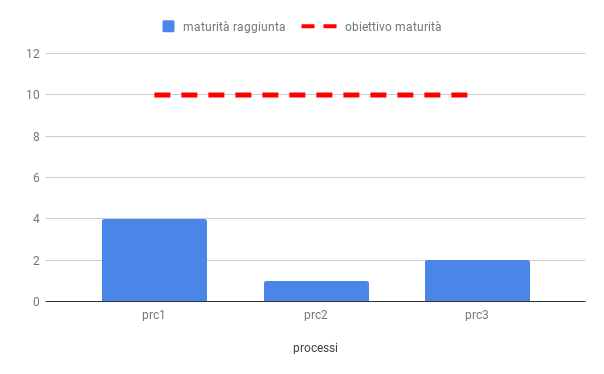
\includegraphics[scale=0.5]{MaturitaProcessi.png}
	\caption{Maturità macro-processi ISO 15504}
\end{figure}
\begin{itemize}
	\item \textbf{prc1:} processo gestito da automatismi, il gruppo sta imparando ad utilizzare quest'ultimi per rendere il lavoro più preciso e con meno possibilità di errore. Usando ad esempio toggle per il conteggio ore e integrazione slack con github tracciando le issue ha
	permesso di ottenere una migliore pianificazione;
	\item \textbf{proc2:} processo non ancora istanziato poichè non fa parte della revisione di requisit, abbiamo analizzato solo metriche in funzione degli obiettivi;
	\item \textbf{proc3:} processo non ancora istanziato, sarà comunque quasi completamente automatizzato
\end{itemize}
\clearpage
\subsubsection{Qualità di prodotto}
In questa fase ci si concentra principalmente sulla redazione dei documenti, pertanto le uniche metriche utilizzate sono quelle riguardanti i documenti.
Poichè, in particolari circostanze (non necessariamente rare), la valutazione automatica della leggibilità, se non tiene conto in alcun modo dei significati delle parole, può dare risultati inattendibili, per non dire fuorvianti si è scelto di non valutare i documenti tramite script che calcolano le metriche.
Nonostante cioò sono metriche puramente sintattiche, sono da considerare con la dovuta cautela \\
\href{https://docs.google.com/spreadsheets/d/1yMKJyV4I8FXQ7GUQOq8m1RdZeTYFTJ387ixzofNrfLI/edit?usp=sharing}{modifica grafici}\\
\href{https://www.webfx.com/tools/read-able/check.php?tab=Test+By+Url&uri=https%3A%2F%2Fwww.ispazio.net}{prova test leggibilità}
	 \\ \\
	Come si può notare dal trend dei grafici l'obiettivo è stato quasi sempre rispettato ottenendo dei documenti con una leggibilità media da istruzione superiore.
	\clearpage
\paragraph{Gunning Fog index}
\hspace{15cm}
\begin{figure}[h!]
	\centering
	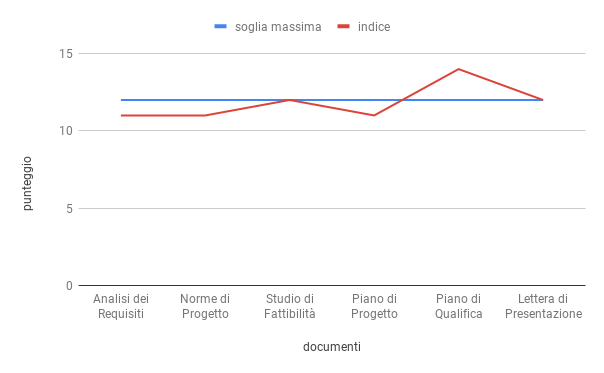
\includegraphics[scale=0.5]{GunningFogIndex.png}
	\caption{Gunning Fog index}

\end{figure}
%\clearpage
\paragraph{Simple Measure of Gobbledygook (SMOG)}
\hspace{15cm}
\begin{figure}[h!]
	\centering
	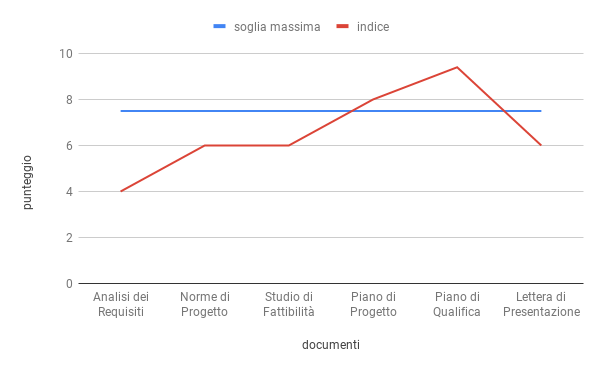
\includegraphics[scale=0.5]{Smog.png}
	\caption{SMOG}
\end{figure}
\clearpage
\paragraph{Gulpease Index}
\hspace{15cm}
\begin{figure}[h!]
	\centering
	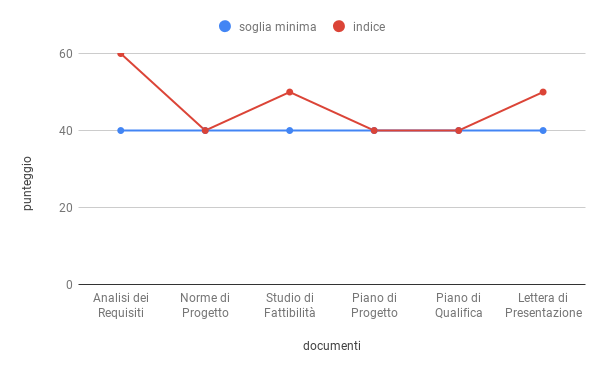
\includegraphics[scale=0.5]{GulpeaseIndex.png}
	\caption{Gulpease index}
\end{figure}

\paragraph{Errori sintattici}
\hspace{15cm}
 I verificatori hanno eliminato gli errori rimanenti presenti nei documenti, raggiungendo così il valore ottimale prefissato attraverso il software per il controllo ortografico presente in TexStudio. 
\subsubsection{Conclusioni}
Parlare se si è sforati nel budget (parlare quindi di metriche per il budget) e in quel caso perchè è successo.
\clearpage
\subsection{Revisione di Progettazione (RP)}
Questa sezione verrà riempita durante il periodo definito.
\subsection{Revisione di Qualifica(RQ)}
Questa sezione verrà riempita durante il periodo definito
\subsection{Revisione di Accettazione(RA)}
Questa sezione verrà riempita durante il periodo definito
\newpage
\section{Test di unità}
\textbf{Lo mettiamo e diciamo che lo facciamo più avanti, tanto per far capire la natura incrementale del documento}
\newpage
\section{Test di integrazione}
Questa sezione verra' sviluppata in seguito quando sara' richista la sua istanziazione
\newpage
\end{document}